\documentclass[twoside,10pt]{article}
\usepackage{/Users/bradenhoagland/latex/styles/toggles}
%\toggletrue{sectionbreaks}
%\toggletrue{sectionheaders}
\newcommand{\docTitle}{Knot Groups and the Wirtinger Presentation}
\usepackage{/Users/bradenhoagland/latex/styles/common}
\importStyles{formal}{rainbow}{plain}

\usepackage[
        backend=biber,
]{biblatex}
\addbibresource{bib.bib}

%\renewcommand{\theenumi}{\alph{enumi}}

\begin{document}
%\tableofcontents

\formalTitle{\docTitle}{Braden Hoagland}{Math 323S: Geometry}

\formalHeader{Braden Hoagland}{Knot Groups}

%--------------------------------------------------------------------------------
% Introduction
%--------------------------------------------------------------------------------
\section{Introduction}

Mathematical knots are idealized notions of real-life knots: instead of a thick piece of rope of finite length, we use an infinitesimally thin line with ends fused together. Below are a few examples; the first two are well known knots called  the unknot and the trefoil knot.

\begin{figure}[H]
	\centering
	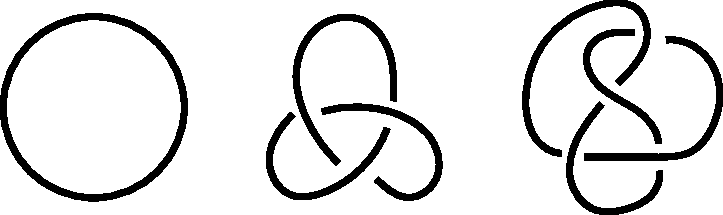
\includegraphics[scale=1]{fig/knots.pdf}
	%\caption{}
\end{figure}

Looking at examples, it is visually clear that some knots are more complicated than other knots. For instance, the unknot has no twists in it while the others do. Formulating this mathematically is far from trivial, however: every knot is homeomorphic to every other knot, so any distinguishing invariant can only be formulated with a bit of creativity.

The aim of this paper is to develop such an invariant: the knot group. We first give a detailed argument for the earlier claim that any two knots are homeomorphic. We then develop some theory regarding the fundamental group and use it to propose a useful knot invariant called the knot group. We conclude by deriving a method to compute it, giving the Wirtinger presentation of the knot group, and we explore several examples to show how useful this presentation is in quickly distinguishing knots.

%--------------------------------------------------------------------------------
% Background
%--------------------------------------------------------------------------------
\section{Background}

A \textbf{knot} $K$ is an embedding of the circle $S^{1}$ in $\R^{3}$, i.e. the image of a continuous injection $f:S^{1}\to \R^{3}$. As in many branches of mathematics, we want to find some invariant that allows us tell different knots apart. To motivate the particular invariant discussed in this paper (the knot group), we can consider what goes wrong when we analyze a knot without paying attention to its ambient space $\R^{3}$.

We claim that any knot $K$ is homeomorphic to $S^{1}$. To see this, we will need several lemmas.


\begin{lem}
	\label{closed-compact}
Any closed subset of a compact space is compact.
\end{lem}
\begin{proof}
	Suppose $A$ is a closed subset of a compact set $X$, and suppose $\mathcal{U}$ is an open cover of $A$. Since $A$ is closed, $\mathcal{U} \uni (X-A)$ is an open cover of $X$. Since $X$ is compact, this cover has a finite subcover $\left\{ U_1, \dots, U_n, X-A \right\}$, where each $U_i$ is in $\mathcal{U}$. But then $\left\{ U_1, \dots, U_n \right\}$ is necessarily a finite subcover of $\mathcal{U}$, so $A$ is compact.
\end{proof}

\begin{lem}
	\label{compact-haus}
Any compact subset of a Hausdorff space is closed.
\end{lem}
\begin{proof}
	Suppose $A$ is a compact subset of a Hausdorff space $X$. We will show that $X-A$ is open. Fix $x \in X-A$, then for all $a \in A$, there are disjoint neighborhoods $U_a$ of $a$ and $V_{a}$ of $x$ since $X$ is Hausdorff.

	Note that $\left\{ U_a \right\}_{a\in A}$ is an open cover of $A$, so since $A$ is compact, it has a finite subcover $\left\{ U_{a_i} \right\}_{i=1}^{n}$. Then $\bigcap_{i=1}^{n}V_{a_i}$ is an open neighborhood of $x$ (it's open since the intersection is finite) that does not intersect $A$. Since $x$ was arbitrary, $X-A$ is open, so $A$ is closed.
\end{proof}

\begin{lem}
	\label{bij-closed-homeo}
A continuous map is \textbf{closed} if it sends closed sets to closed sets. A bijective closed map is a homeomorphism.
\end{lem}
\begin{proof}
	Suppose $f:X\to Y$ is a closed bijection, then we can clearly define an inverse $f^{-1}:Y\to X$. To show that it is continuous, note that for $U$ closed in $X$, $(f^{-1})^{-1}(U) = f(U)$ is closed in $Y$ since $f$ is a closed map.
\end{proof}

\begin{lem}
	\label{compact-haus-homeo}
Suppose $f:X\to Y$ is a continuous bijection, $X$ is compact, and $Y$ is Hausdorff. Then $f$ is a homeomorphism.
\end{lem}
\begin{proof}
	Let $A$ be a closed set of $X$, then since $X$ is compact, $A$ is also compact by \Cref{closed-compact}. Since continuous maps preserve compactness, $f(A)$ is a compact subset of $Y$. Since $Y$ is Hausdorff, it is closed by \Cref{compact-haus}. Thus $f$ is a closed map. Then by \Cref{bij-closed-homeo}, $f$ is a homeomorphism.
\end{proof}

\begin{thrm}[]
	Every knot is homeomorphic to $S^{1}$.
\end{thrm}
\begin{proof}
	Suppose $K$ is the image of continuous injection $f:S^{1}\to \R^{3}$. Note that $K$ is Hausdorff with the subspace topology inherited from $\R^{3}$, and also note that $f$ necessarily maps onto $K$. Since $S^{1}$ is compact, $S^{1}\cong K$ by \Cref{compact-haus-homeo}.
\end{proof}

The main philosophical consequence of this theorem is that, topologically speaking, any two knots are the same. Thus if we want a topological invariant for a knot, it will have to somehow include the ambient space $\R^{3}$. Perhaps the most straightforward way of doing this is, given a knot $K$, analyzing $\R^{3}-K$ instead of $K$.

%-------------------
% Knot Groups
%-------------------
\subsection{Knot Groups}

To determine how complex $K$ is, we will study the space of homotopy classes of loops of $\R^{3}-K$, i.e. the fundamental group of $\R^{3}-K$. We'll need a few basic definitions before we do this.

Suppose $f,g:X\to Y$ are two continuous maps, then a \textbf{homotopy} between $f$ to $g$ is a continuous map $H:X\times I \to Y$, where $I=[0,1]$, such that $H(\cdot,0) = f$ and $H(\cdot,1)$. If a homotopy exists between $f$ and $g$, we say they are \textbf{homotopic} and denote this by $f \simeq g$.

We can extend homotopies to work with loops instead of general maps. We define a \textbf{loop} in $X$ to be a continuous map $S^{1}\to X$. Suppose we denote a special basepoint $0 \in S^{1}$, then we say that a loop $f$ is \textbf{based at} $0$ if $f(0)$. We can ``multiply" two loops $f$ and $g$ (both based at the same point) by concatenating them.

If we have two loops $f$ and $g$ based at the same point, then a \textbf{homotopy of loops} between them is a standard homotopy $H$ with the added restriction that $H(0,t) = f(0)=g(0)$ for all $t \in I$.

Then given a space $X$, we can partition the set of loops based at $x \in X$ with the equivalence relation given by $f \simeq g \iff f$ and $g$ are loop homotopic. From now on, we will use the notation $[f]$ to denote the equivalence class of $f$. We can finally define the fundamental group.

\begin{defn}[]
	Suppose $X$ is a topological space. Then the \textbf{fundamental group} $\pi_1(X,x)$ of $X$ based at $x$ is the set
	\[
		\Big\{ [f] \;\Big|\; f \text{ is a loop based at } x \Big\}
	\] equipped with the group operation of path multiplication.
\end{defn}

The fundamental group is a useful tool for distinguishing topological spaces since it is a topological invariant. But one annoying part of the definition is its reliance on a basepoint. Luckily, we don't have to worry about this when working with knots.

\begin{prop}
Any two fundamental groups in a path connected space are isomorphic.
\end{prop}
\begin{proof}
	Consider $\pi_1(X,x_0)$ and $\pi_1(X,x_1)$. Suppose $X$ is path connected, then there is a path $h$ from $x_0$ to $x_1$. Then the map
        \begin{align*}
                \pi_1(X,x_1) &\to \pi_1(X,x_0) \\
                [f] &\mapsto [h f \overline{h}].
        \end{align*}
	is a group homomorphism with inverse $[f] \mapsto [\overline{h}fh]$. Thus it is also an isomorphism.
\end{proof}

By Theorem 4 in \cite{hur}, the knot complement $\R^{3}-K$ is path connected. Thus we can define the \textbf{knot group} of $K$ to be (up to isomorphism) the fundamental group $\pi_1(\R^{3}-K, x)$ for any $x \in \R^{3}-K$. Since the basepoint is inconsequential, we will drop it from our notation from now on.

As a final note, we can treat $\pi_1$ as a covariant functor $\cat{Top}_*\to \cat{Grp}$, which can be checked routinely. This fact will significantly clean up a few later proofs. Note that although the next theorem assumes path connectedness, this assumption is unnecessary and only used to clean up notation.

\begin{thrm}[]
	$\pi_1$ is a covariant functor mapping $X \to \pi_1(X,x_0)$ and $f:X\to Y$ to the group homomorphism
	\begin{align*}
		f_{*}: \pi_1(X) &\to \pi_1(Y) \\
		[\alpha] &\mapsto [f\alpha].
	\end{align*}
\end{thrm}

This functor plays nicely with homotopic maps, too: it sends them to the same induced homomorphism, which we present without proof due to the technical machinery needed to build up to this result.

\begin{prop}
	\label{homotopic-same-induced}
If $f \simeq g$, the $f_* = g_*$.
\end{prop}

Although it has a sound theoretical backing, knot groups would ultimately be useless if we could not compute them. Luckily, their computation is straightforward, allowing for the calculation of knot groups of complicated knots with relative ease. To facilitate this computation, we will need to take a brief detour to discuss deformation retractions.

%-------------------
% Deformation Retractions
%-------------------
\subsection{Deformation Retractions}

Suppose $A \subset X$. A \textbf{retraction} of $X$ onto $A$ is a continous map $r:X\to A$ that fixes $A$. Equivalently, $r \circ i = 1_{A}$, where $i:A \inj X$ is the natural inclusion. A \textbf{deformation retraction} of $X$ onto $A$ is then a homotopy between $1_X$ and a retraction $r:X\to A$ that fixes $A$. To be precise, a deformation retraction is a map $F:X\times I \to X$ such that
\begin{align*}
	F(\cdot,0) &= \id_{X}, \\
	F(\cdot,t) &= \id_{A} \quad \forall t, \\
	F(x,1) &\in A \quad \forall x \in X.
\end{align*}

To be precise, this is a homotopy between $1_X$ and $i \circ r$. Thus one can think of deformation retractions as continuously ``shrinking" one space onto a smaller space through time. The most important property of deformation retractions for our purposes is that they preserve fundamental groups.

\begin{thrm}
	\label{DR-homeo}
	Suppose $X$ is path connected and deformation retracts onto $A$, then $\pi_1(X) \cong \pi_1(A)$.
\end{thrm}
\begin{proof}
	First note that $r := F(\cdot,1)$ is a retraction onto $A$. Then since it's continuous, $r(X) = A$ is also path connected, and so it makes sense to refer to both $\pi_1(X)$ and $\pi_1(A)$ without basepoints. Now we can apply the $\pi_1$ functor to the following commutative diagram.
	\[
	\begin{tikzcd}
		A \rar[hook, shift left]{i} & X \lar[two heads, shift left]{r} & \leadsto & \pi_1(A) \rar[hook, shift left]{i_{*}} & \pi_1(X) \lar[two heads, shift left]{r_{*}}
	\end{tikzcd}
	\] 
	Note that by functoriality, the second diagram shows $r_{*}i_{*} = (ri)_{*} = (\id_{A})_{*}=\id_{\pi_1(A)}$. To show the other half of the isomorphism, note that the deformation retraction shows $i \circ r \simeq \id_{X}$. Then by \Cref{homotopic-same-induced}, $i_{*}r_{*} = (ir)_{*} = (\id_{X})_{*} = \id_{\pi_1(X)}$. Thus $\pi_1(A) \cong \pi_1(X)$.
\end{proof}


%--------------------------------------------------------------------------------
% The Wirtinger Presentation
%--------------------------------------------------------------------------------
\section{The Wirtinger Presentation}

The main idea of the Wirtinger presentation is to find a deformation retraction of $\R^{3}-K$ in which it's easier to compute the fundamental group. Then by \Cref{DR-homeo}, this is the same as $\pi_1(\R^{3}-K)$.

Suppose we lie our knot $K$ on a flat surface, then we can examine each crossing individually. Suppose we've oriented a crossing as below, then we can take rectangular strips $R_i, R_j$, and $R_k$ and lie them over each of the three distinct segments to form tunnels, fusing their edges into the surface. We also fuse together each of the tunnels at the four designated points.

\begin{figure}[H]
	\centering
	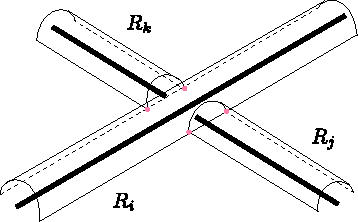
\includegraphics[scale=1.5]{fig/rectangles.pdf}
	%\caption{}
\end{figure}

Now take a square $S_{\ell}$ and place it on top of the crossing, fusing it together with the tunnels as shown. With a bit of thought, one can see that this is a deformation retract of $\R^{3}-K$, and thus it must have the same fundamental group.

\begin{figure}[H]
	\centering
	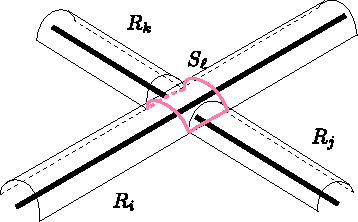
\includegraphics[scale=1.5]{fig/with-square.pdf}
	%\caption{}
\end{figure}

It is straightforward to find this space's fundamental group. For a single crossing, remove $S_{\ell}$, then there are three distinct classes of loops, each going around a different tunnel. At this point, the fundamental group is free with a generator $x_i$ for each $R_i$.

Now orient the segments as below; a bit of thought shows that this orientation can be carried on throughout the rest of the crossings in a compatible way. Then for any loop going around a rectangular strip, we can orient it via the right hand rule.

\begin{figure}[H]
	\centering
	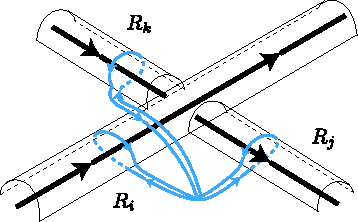
\includegraphics[scale=1.5]{fig/orient.pdf}
	%\caption{}
\end{figure}

Now add in $S_\ell$ again. Based on the orientation we just decided on, $S_\ell$ is a 2-cell with the following orientations on each edge.

\begin{figure}[H]
	\centering
	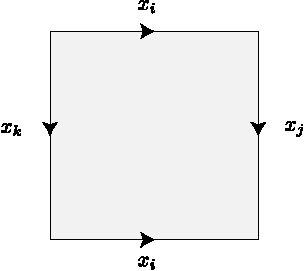
\includegraphics[scale=1]{fig/square-orient.pdf}
	%\caption{}
\end{figure}

By Van Kampen's Theorem, this adds in relations of the form $x_i x_j x_i^{-1} x_k^{-1} = 1$ to the fundamental group. Thus the knot group of any knot has a generator $x_i$ for each distinct segment and a relation $x_i x_j x_i^{-1} = x_k$ for each crossing. This presentation of the group is the \textbf{Wirtinger presentation}, and we can see its computational benefits firsthand through the following two examples.

\begin{ex}[The unknot]
	Suppose $K$ is an unknot, then it has one distinct segment and no crossings. This means its knot group has one generator and no added relations, i.e. $\pi_1(\R^{3}-K) \cong \mathbb{Z}$.

	\begin{figure}[H]
		\centering
		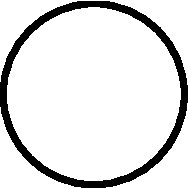
\includegraphics[scale=1]{fig/unknot.pdf}
		%\caption{}
	\end{figure}
\end{ex}

\newpage

\begin{ex}[The trefoil knot]
	Suppose $K$ is a trefoil knot, then it has three distinct segments and three crossings.
	\begin{figure}[H]
		\centering
		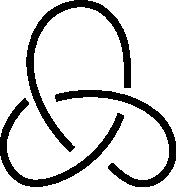
\includegraphics[scale=1]{fig/trefoil.pdf}
		%\caption{}
	\end{figure}
Thus its knot group is
\[
	\pi_1(\R^{3}-K) \cong \ang{x_1,x_2,x_3 \;|\; x_1x_2x_1^{-1}=x_3, \; x_2x_3x_2^{-1}=x_1, \; x_3x_1x_3^{-1}=x_2}.
\]
Note that we can express $x_3$ in terms of $x_1$ and $x_3$. Doing so, all relations simplify to the same one, giving
\[
\ang{x_1,x_2 \;|\; x_1x_2x_1 = x_2x_1x_2}.
\] 
From here we can make two different notational simplications, each yielding a common presentation of the trefoil knot's knot group. If we let $a=x_1$ and $b=x_2$, then this becomes
\[
\ang{a,b \;|\; aba=bab}.
\] This isn't a particularly substantive change, just a cosmetic one. Alternatively, if we let $a = x_1x_2x_1$ and $b=x_2x_1$, then $a_3 = x_1x_2x_1x_2x_1x_2 = (x_2x_1x_2)(x_1x_2x_1) = b^{3}$. Thus an equivalent presentation of the knot group is
\[
\ang{a,b \;|\; a^{2}=b^{3}}.
\] In fact, we can generalize this argument in a straightforward way to apply to $(p,q)$-torus knots, where $p$ and $q$ are relatively prime. In this general case, the knot group ends up being
\[
\ang{a, b \;|\; a^{p}= b^{q}}.
\] 
\end{ex}


%--------------------------------------------------------------------------------
% Bibliography
%--------------------------------------------------------------------------------
\nocite{hatcher}
\nocite{linov}
\nocite{ncat}

\printbibliography


\end{document}
